\subsection{Светодиод WS2812b}

Существует большое количество разновидностей адресных светодиодов. Одним из самых популярных является WS2812b.

WS2812 представляет из себя адресный светодиод, состоящий из контроллера и RGB чипа, интегрированных в светодиод SMD 5050. Также он включает в себя обработчик цифровых данных и контроллер восстановления и усиления сигнала~\cite{Worldseim}.

Основные эталонные характеристики светодиода WS2812b:

\begin{enumerate}
  \item Размер --- 5х5 мм;
  \item Частота ШИМ --- 400Гц;
  \item Напряжение питания --- $+3.5 \sim 5.3$ В;
  \item Потребление при нулевой яркости --- 1 мА на светодиод;
  \item Потребление при максимальной яркости --- 60 мА на светодиод;
  \item Номинальный световой поток --- 16 Люмен;
  \item Рабочая температура --- $-25^\circ C \sim +80^\circ C$;
  \item Цветность: RGB, 256 оттенков на канал, 16 миллионов цветов;
  \item Размер данных --- 24 бита на светодиод;
  \item Скорость передачи данных --- 800 кГц.
\end{enumerate}

На рисунке~\ref{img:WS2812__schema} представлено схематическое изображение светодиода WS2812b, назначение выводов светодиода представлено в таблице~\ref{tab:ws2812__pin}, на рисунке~\ref{img:WS2812__strip} представлена базовая схема светодиодной ленты, основанной на WS2812b~\cite{Worldseim}.

\begin{figure}[H]
  \centering
  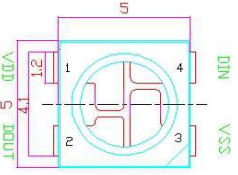
\includegraphics[height=0.2\textheight]{assets/images/theoretical/Схема светодиода.png}
  \caption{Схематическое изображение светодиода WS2812b}
  \label{img:WS2812__schema}
\end{figure}

\begin{table}[H]
  \caption{Назначение выводов светодиода WS2812b}
  \label{tab:ws2812__pin}
  \begin{tabular}{|c|c|l|}
  \hline
  Номер & Обозначение & Описание функции \\ \hline
  1 & VDD  & Подача питания светодиода            \\ \hline
  2 & DOUT & Вывод сигнала управляющей информации \\ \hline
  3 & VSS  & Заземление                           \\ \hline
  4 & DIN  & Ввод сигнала управляющей информации  \\ \hline
  \end{tabular}
  \end{table}

\begin{figure}[H]
  \centering
  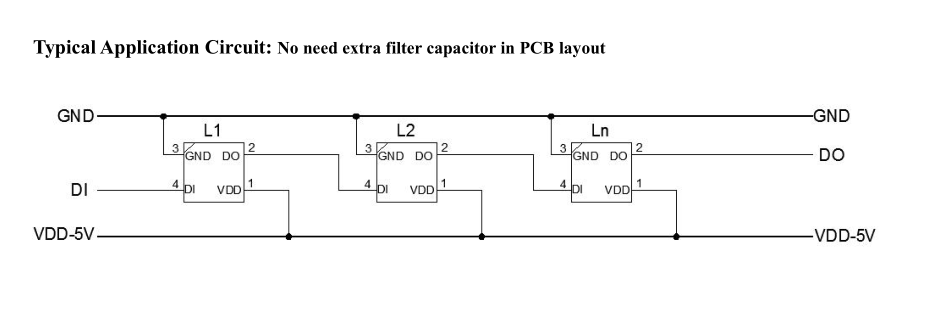
\includegraphics[height=0.2\textheight]{assets/images/theoretical/Базовая схема светодиодной ленты.png}
  \caption{Базовая схема светодиодной ленты, основанной на WS2812b}
  \label{img:WS2812__strip}
\end{figure}


В протокол передачи данных применяется линейное кодирование NRZ, код без возвращения к нулю. То есть, при передаче информации на расстояние информация представляется в цифровом виде и в канал связи формируется сигнал в соответствии с кодом: логическому нулю соответствует нижний уровень сигнала, логической единице соответствует верхний уровень сигнала; информационные переходы происходят на границах значащего интервала. После того, как на ленту светодиодов подаётся питание, вход DIN получает информацию от управляющего устройства, первый светодиод получает начальные 24 бита информации, соответствующие последовательно идущим 8 битам каждого из цветов RGB, и подаёт эти данные на обработчик информации. После этого оставшиеся данные, то есть данные, полученные на DIN без первых 24 бит, восстанавливаются  с помощью внутреннего контроллера восстановления сигнала и передаются на выход DO светодиода. Канал DIN следующего светодиода считывает данные из выхода DO предыдущего, и процесс повторяется~\cite{Worldseim}. Таким образом, количество светодиодов в ленте неограниченно и зависит только от скорости передачи сигнала. На рисунке~\ref{img:WS2812__data_transmission} представлена временная диаграмма передачи данных в ленте светодиодов.

\begin{figure}[H]
  \centering
  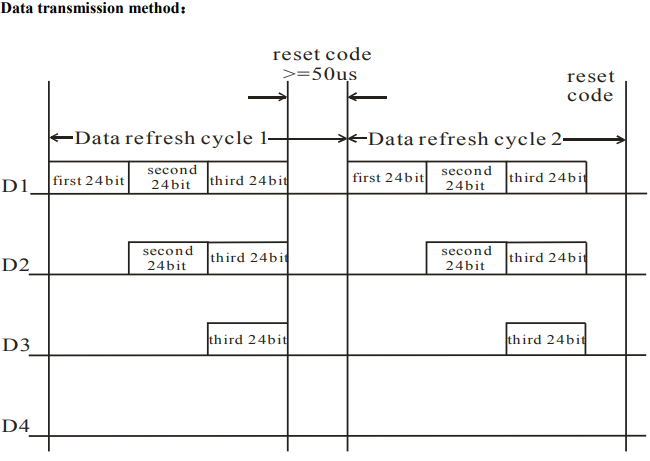
\includegraphics[width=0.6\textwidth]{assets/images/theoretical/Временная диаграма передачи данных.png}
  \caption{Временная диаграмма передачи данных в ленте светодиодов}
  \label{img:WS2812__data_transmission}
\end{figure}
